\documentclass[]{elsarticle} %review=doublespace preprint=single 5p=2 column
%%% Begin My package additions %%%%%%%%%%%%%%%%%%%
\usepackage[hyphens]{url}
\usepackage{lineno} % add
\providecommand{\tightlist}{%
  \setlength{\itemsep}{0pt}\setlength{\parskip}{0pt}}

\bibliographystyle{elsarticle-harv}
\biboptions{sort&compress} % For natbib
\usepackage{graphicx}
\usepackage{booktabs} % book-quality tables
\usepackage[font=small]{caption}
\usepackage[labelformat = empty,position=top]{subcaption}
\usepackage[export]{adjustbox}

%% Redefines the elsarticle footer
%\makeatletter
%\def\ps@pprintTitle{%
% \let\@oddhead\@empty
% \let\@evenhead\@empty
% \def\@oddfoot{\it \hfill\today}%
% \let\@evenfoot\@oddfoot}
%\makeatother

\newcommand{\subfigimg}[3][,]{%
	\setbox1=\hbox{\includegraphics[#1]{#3}}% Store image in box
	\leavevmode\rlap{\usebox1}% Print image
	\rlap{\hspace*{10pt}\raisebox{\dimexpr\ht1-2\baselineskip}{#2}}% Print label
	\phantom{\usebox1}% Insert appropriate spcing
}

% A modified page layout
\textwidth 6.75in
\oddsidemargin -0.15in
\evensidemargin -0.15in
\textheight 9in
\topmargin -0.5in
%%%%%%%%%%%%%%%% end my additions to header

\usepackage[T1]{fontenc}
\usepackage{lmodern}
\usepackage{amssymb,amsmath}
\usepackage{ifxetex,ifluatex}
\usepackage{fixltx2e} % provides \textsubscript
% use upquote if available, for straight quotes in verbatim environments
\IfFileExists{upquote.sty}{\usepackage{upquote}}{}
\ifnum 0\ifxetex 1\fi\ifluatex 1\fi=0 % if pdftex
  \usepackage[utf8]{inputenc}
\else % if luatex or xelatex
  \usepackage{fontspec}
  \ifxetex
    \usepackage{xltxtra,xunicode}
  \fi
  \defaultfontfeatures{Mapping=tex-text,Scale=MatchLowercase}
  \newcommand{\euro}{€}
\fi
% use microtype if available
\IfFileExists{microtype.sty}{\usepackage{microtype}}{}
\usepackage{color}
\usepackage{fancyvrb}
\newcommand{\VerbBar}{|}
\newcommand{\VERB}{\Verb[commandchars=\\\{\}]}
\DefineVerbatimEnvironment{Highlighting}{Verbatim}{commandchars=\\\{\}}
% Add ',fontsize=\small' for more characters per line
\usepackage{framed}
\definecolor{shadecolor}{RGB}{248,248,248}
\newenvironment{Shaded}{\begin{snugshade}}{\end{snugshade}}
\newcommand{\KeywordTok}[1]{\textcolor[rgb]{0.13,0.29,0.53}{\textbf{{#1}}}}
\newcommand{\DataTypeTok}[1]{\textcolor[rgb]{0.13,0.29,0.53}{{#1}}}
\newcommand{\DecValTok}[1]{\textcolor[rgb]{0.00,0.00,0.81}{{#1}}}
\newcommand{\BaseNTok}[1]{\textcolor[rgb]{0.00,0.00,0.81}{{#1}}}
\newcommand{\FloatTok}[1]{\textcolor[rgb]{0.00,0.00,0.81}{{#1}}}
\newcommand{\ConstantTok}[1]{\textcolor[rgb]{0.00,0.00,0.00}{{#1}}}
\newcommand{\CharTok}[1]{\textcolor[rgb]{0.31,0.60,0.02}{{#1}}}
\newcommand{\SpecialCharTok}[1]{\textcolor[rgb]{0.00,0.00,0.00}{{#1}}}
\newcommand{\StringTok}[1]{\textcolor[rgb]{0.31,0.60,0.02}{{#1}}}
\newcommand{\VerbatimStringTok}[1]{\textcolor[rgb]{0.31,0.60,0.02}{{#1}}}
\newcommand{\SpecialStringTok}[1]{\textcolor[rgb]{0.31,0.60,0.02}{{#1}}}
\newcommand{\ImportTok}[1]{{#1}}
\newcommand{\CommentTok}[1]{\textcolor[rgb]{0.56,0.35,0.01}{\textit{{#1}}}}
\newcommand{\DocumentationTok}[1]{\textcolor[rgb]{0.56,0.35,0.01}{\textbf{\textit{{#1}}}}}
\newcommand{\AnnotationTok}[1]{\textcolor[rgb]{0.56,0.35,0.01}{\textbf{\textit{{#1}}}}}
\newcommand{\CommentVarTok}[1]{\textcolor[rgb]{0.56,0.35,0.01}{\textbf{\textit{{#1}}}}}
\newcommand{\OtherTok}[1]{\textcolor[rgb]{0.56,0.35,0.01}{{#1}}}
\newcommand{\FunctionTok}[1]{\textcolor[rgb]{0.00,0.00,0.00}{{#1}}}
\newcommand{\VariableTok}[1]{\textcolor[rgb]{0.00,0.00,0.00}{{#1}}}
\newcommand{\ControlFlowTok}[1]{\textcolor[rgb]{0.13,0.29,0.53}{\textbf{{#1}}}}
\newcommand{\OperatorTok}[1]{\textcolor[rgb]{0.81,0.36,0.00}{\textbf{{#1}}}}
\newcommand{\BuiltInTok}[1]{{#1}}
\newcommand{\ExtensionTok}[1]{{#1}}
\newcommand{\PreprocessorTok}[1]{\textcolor[rgb]{0.56,0.35,0.01}{\textit{{#1}}}}
\newcommand{\AttributeTok}[1]{\textcolor[rgb]{0.77,0.63,0.00}{{#1}}}
\newcommand{\RegionMarkerTok}[1]{{#1}}
\newcommand{\InformationTok}[1]{\textcolor[rgb]{0.56,0.35,0.01}{\textbf{\textit{{#1}}}}}
\newcommand{\WarningTok}[1]{\textcolor[rgb]{0.56,0.35,0.01}{\textbf{\textit{{#1}}}}}
\newcommand{\AlertTok}[1]{\textcolor[rgb]{0.94,0.16,0.16}{{#1}}}
\newcommand{\ErrorTok}[1]{\textcolor[rgb]{0.64,0.00,0.00}{\textbf{{#1}}}}
\newcommand{\NormalTok}[1]{{#1}}
\usepackage{graphicx}
% We will generate all images so they have a width \maxwidth. This means
% that they will get their normal width if they fit onto the page, but
% are scaled down if they would overflow the margins.
\makeatletter
\def\maxwidth{\ifdim\Gin@nat@width>\linewidth\linewidth
\else\Gin@nat@width\fi}
\makeatother
%\let\Oldincludegraphics\includegraphics
%\renewcommand{\includegraphics}[1]{\Oldincludegraphics[width=\maxwidth]{#1}}
\ifxetex
  \usepackage[setpagesize=false, % page size defined by xetex
              unicode=false, % unicode breaks when used with xetex
              xetex]{hyperref}
\else
  \usepackage[unicode=true]{hyperref}
\fi
\hypersetup{breaklinks=true,
            bookmarks=true,
            pdfauthor={},
            pdftitle={Carrying Capacity Optimal Escapement},
            colorlinks=true,
            urlcolor=blue,
            linkcolor=magenta,
            pdfborder={0 0 0}}
\urlstyle{same}  % don't use monospace font for urls
\setlength{\parindent}{0pt}
\setlength{\parskip}{6pt plus 2pt minus 1pt}
\setlength{\emergencystretch}{3em}  % prevent overfull lines
\setcounter{secnumdepth}{0}
% Pandoc toggle for numbering sections (defaults to be off)
\setcounter{secnumdepth}{0}
% Pandoc header


\usepackage[nomarkers]{endfloat}

\begin{document}
\begin{frontmatter}

  \title{Optimal harvest strategies in traditional stochastic fisheries models reduce expected yield}
    \author[CEED,UQ]{Matthew Holden\corref{c1}}
   \ead{m.holden1@uq.edu.au} 
   \cortext[c1]{Corresponding Author}
    \author[UCB]{Carl Boettiger}
   \ead{cboettig@gmail.com} 
	\address[CEED]{ARC Centre of Excellence for Environmental Decisions, University of
		Queensland, Brisbane, QLD, 4072, Australia}
    \address[UQ]{Centre for Biodiversity and Conservation Science, University of Queensland, School of Biology, Brisbane, QLD, 4072, Australia}
    \address[UCB]{University of California Berkeley}
  
  \begin{abstract}

  \end{abstract}
  
 \end{frontmatter}

\emph{Text based on elsarticle sample manuscript, see
\url{http://www.elsevier.com/author-schemas/latex-instructions\#elsarticle}}

\section{Introduction}
\section{Methods}
Consider the dynamics of a harvested population with biomass $x_t$ at time $t$ governed by the simple stochastic stock recruitment relationship

\begin{equation}
x_{t+1} = z_{t+1}f(x_t  - h_t),
\end{equation}

where $h_t$ is the biomass harvested at time $t$ and $z_{t+1}$ is a strictly positive random variable with mean one. The optimal escapement, $s_t = x_t  - h_t$, is the value $S$ such that $f'(S)=1/\rho$ where $\rho$ is a discrete time discount equal to $1/(1+\delta)$ where $\delta$ is the continuous discount rate \cite{Reed1979}. For nearly all models, commonly used for stock assessment, (including Beverton-Holt, Ricker, and Logistic maps) this produces escapement rules of one half carrying capacity or less \cite{Reed1979,Clark2010}. This seems quite counter-intuitive. There are stocks for which harvest is very low and yet the fish stock is still declining. However, there are models that can produce optimal escapement arbitrarily close to carrying capacity \cite{pella1969}. However, given that fisheries data is often very noisy, which models provide better harvest strategies in real world fisheries management scenarios, especially under the scenario where our models are wrong? 


Consider the following choices for $f$ with growth rate $r$ and carrying capacity $k$: 

Beverton-Holt recruitment
\begin{equation}\label{BH}
f(x) = \frac{(1+r)x}{1 + rx/k}, 
\end{equation}

Hockey-Stick recruitment
\begin{equation}\label{HS}
f(x) = \begin{cases} 
(1+r)x & x < k/(1+r) \\
k & x\geq k/(1+r).
\end{cases}
\end{equation}

Pella Tomlinson recruitment
\begin{equation}\label{SA}
f(x) = x + rx\left(\frac{\phi+1}{\phi}\right)\left(1 - \left[\frac{x}{k}\right]^\phi\right). 
\end{equation}

The Beverton-Holt recruitment function is standard in fisheries dynamics to represent compensatory density dependence. The Hockey-stick model is similar but discontinuous; the population grows at rate $r$, but with abundance abruptly capped at carrying capacity. Pella-Tomlinson represents over-compensatory dynamics where large populations can experience population declines due to intraspecific competition for resources. 

While we start with these three simple cases, many other models for population growth are possible, such as other over-compensatory recruitment curves (e.g. Ricker), or even strong Allee effects (e.g. Allen).

%Ricker recruitment
%\begin{equation}\label{R}
%f(x) = x e^{r  (1 - x/K)  } , 
%\end{equation}
%
%`Allen" recruitment
%\begin{equation}\label{WA}
%f(x) = x e^{r  (1 - x/k)  (x - c) } , 
%\end{equation}

The optimal harvest rule in these models is an escapement strategy, where escapement is the number of individuals that escape harvest. In other words, the manager tries to leave a fixed number of fish in the ocean and this number is called the escapement. The optimal escapement in \eqref{BH} is $\frac{k}{r} ( \sqrt{ \rho (1+r) } - 1)$ and in \eqref{HS} is $k/(1+r)$ as long as $r>\delta$. It is clear that by making $r$ and $\delta$ arbitrarily close to zero with $r>\delta$, \eqref{HS} achieves an optimal escapement arbitrarily close to carrying capacity $k$. 

We consider the case where each of the three models are the true model that generates the biomass data with perfect measurement and lognormally distributed environmental noise. All three models (of which two are incorrect) are then fit against the data. We then compute the optimal escapement using the formulas above with the parameter values resulting from the fitting procedure. We repeat this process under various low and high values of the intrinsic growth rate, and varying degrees of environmental noise.

\section{Results}

If the growth rate is low ($r=0.15$) then the Beverton-Holt model generates near optimal yield as long as environmental stochasiticity is weak. However, under strong noise the Beverton-Holt model generates the least yield, even when Beverton-Holt is the correct model (circles in Fig. \ref{fig:ModelPerfVSig}). The opposite is true for the Hockey-stick model, it performs best (relative to the true model) when the environmental noise is high (triangles in Fig \ref{fig:ModelPerfVSig}), even when it is the incorrect model (Fig \ref{fig:ModelPerfVSig}ac). The Pella-Tomlinson model performs reasonably well for all stochasticity levels and model truths (Crosses in Fig \ref{fig:ModelPerfVSig}).

If the growth rate is high ($r=1$) Then the true model always performs better than the wrong models, even for large environmental noise (Circles in Fig \ref{fig:ModelPerfVSig}d, triangles in Fig \ref{fig:ModelPerfVSig}e, and crosses in Fig \ref{fig:ModelPerfVSig}f ). This is unlike the case when the growth rate was low and Beverton-Holt model performed worse than the other models under high noise, even when it was the true model. 

\begin{figure}[tb]
	\centering
	\begin{subfigure}[t]{0.02\textwidth}
		\textbf{a)}
	\end{subfigure}
	\begin{subfigure}[t]{0.3\textwidth}
		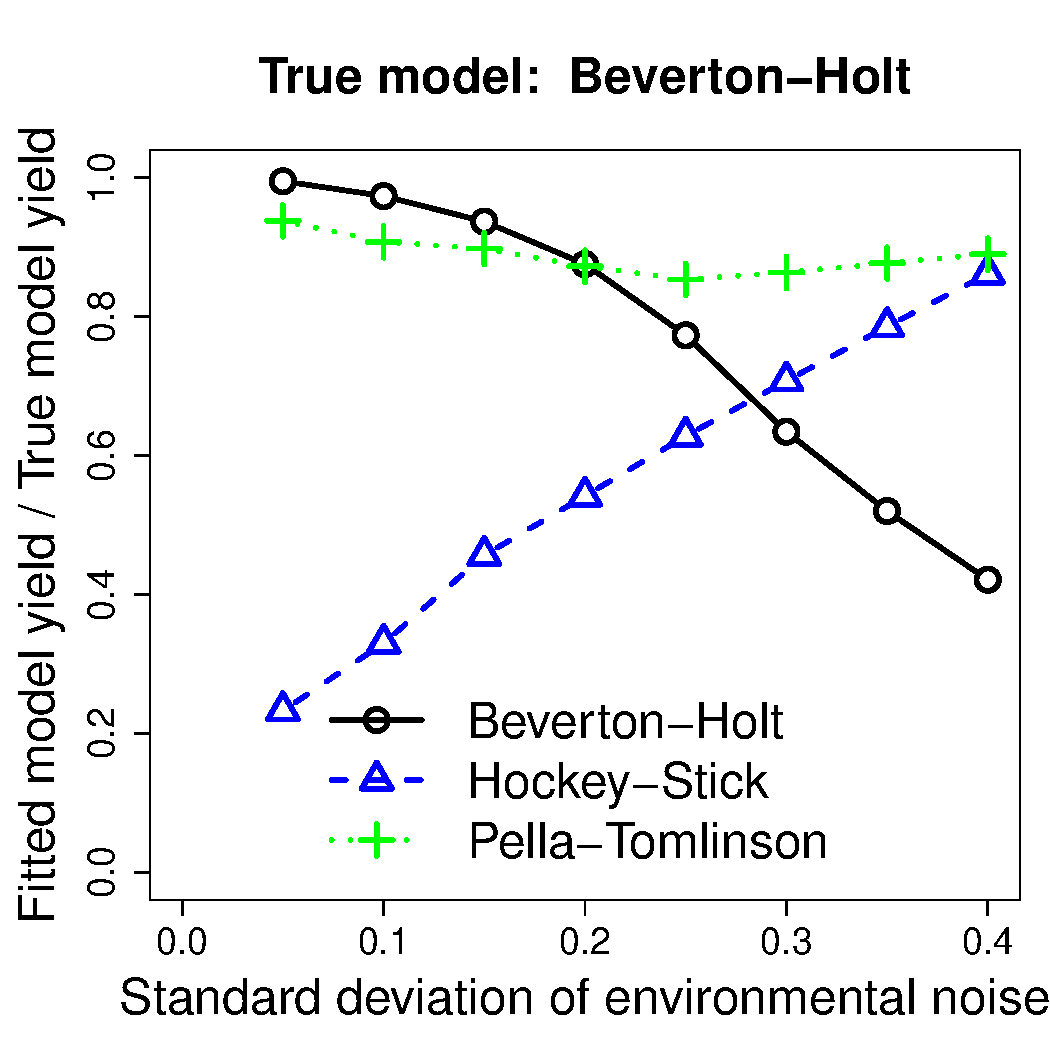
\includegraphics[width=\linewidth,valign=t]{True_1_relativeYield_sim.pdf}
	\end{subfigure}	
	\begin{subfigure}[t]{0.02\textwidth}
		\textbf{b)}
	\end{subfigure}
	\begin{subfigure}[t]{0.3\textwidth}
		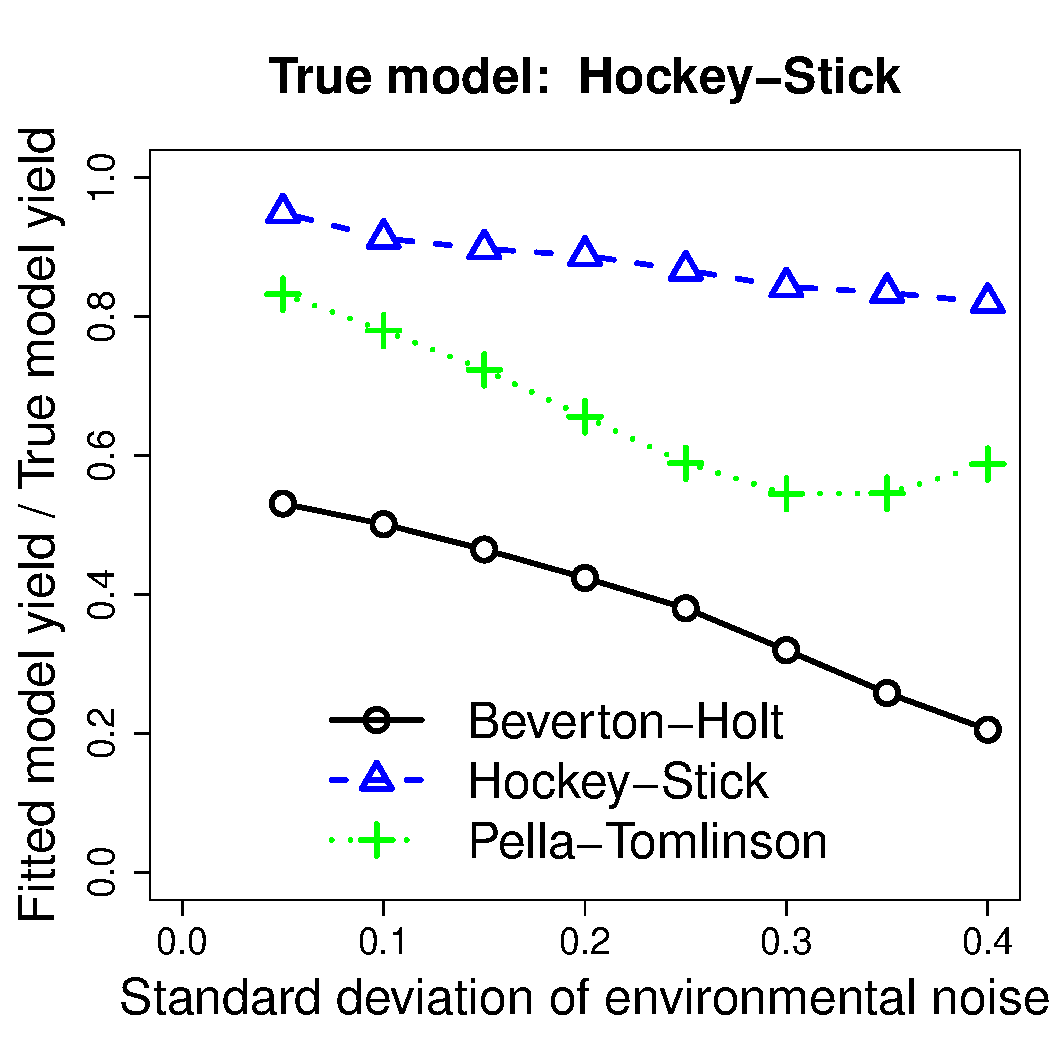
\includegraphics[width=\linewidth,valign=t]{True_2_relativeYield_sim.pdf}
	\end{subfigure}	
	\begin{subfigure}[t]{0.02\textwidth}
		\textbf{c)}
	\end{subfigure}
	\begin{subfigure}[t]{0.3\textwidth}
		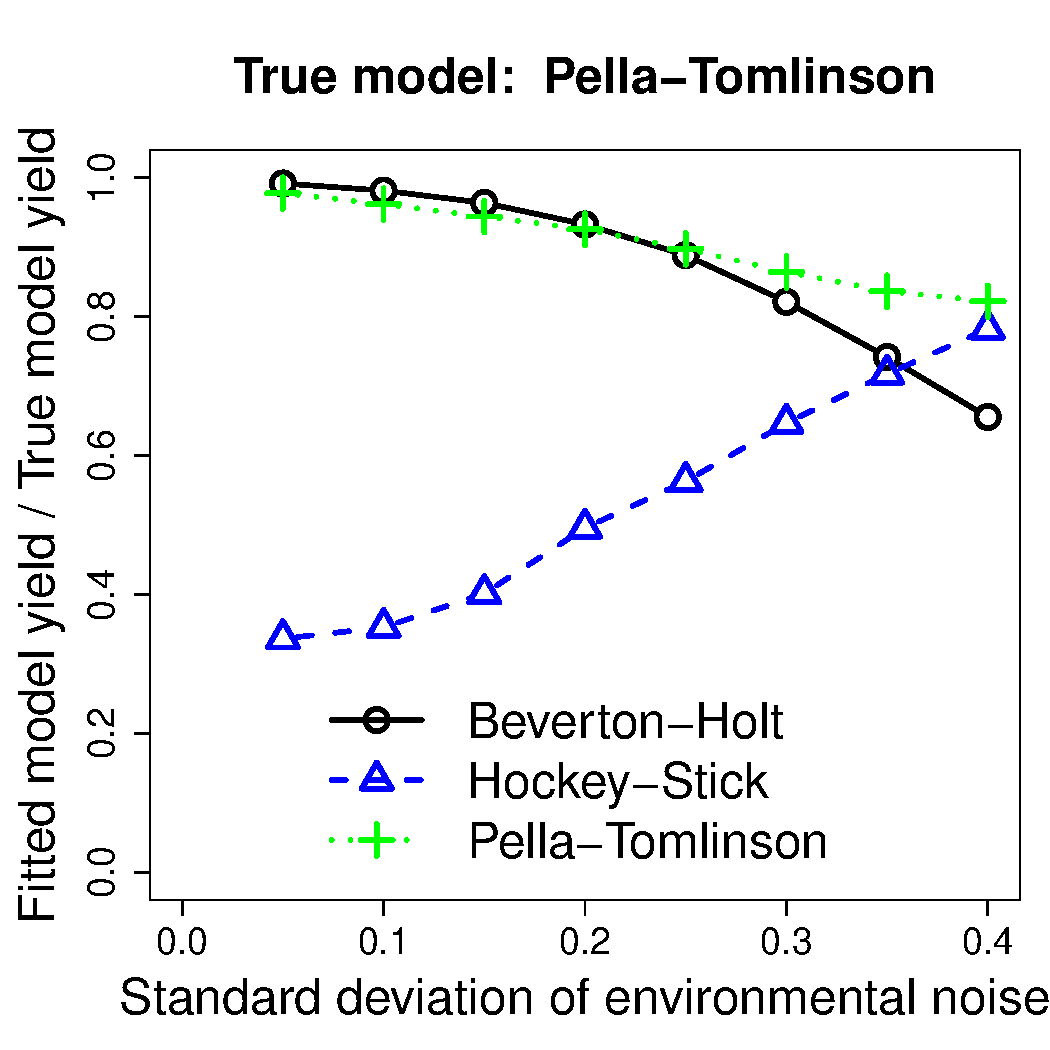
\includegraphics[width=\linewidth,valign=t]{True_3_relativeYield_sim.pdf}
	\end{subfigure}
	\begin{subfigure}[t]{0.02\textwidth}
		\textbf{d)}
	\end{subfigure}
	\begin{subfigure}[t]{0.3\textwidth}
		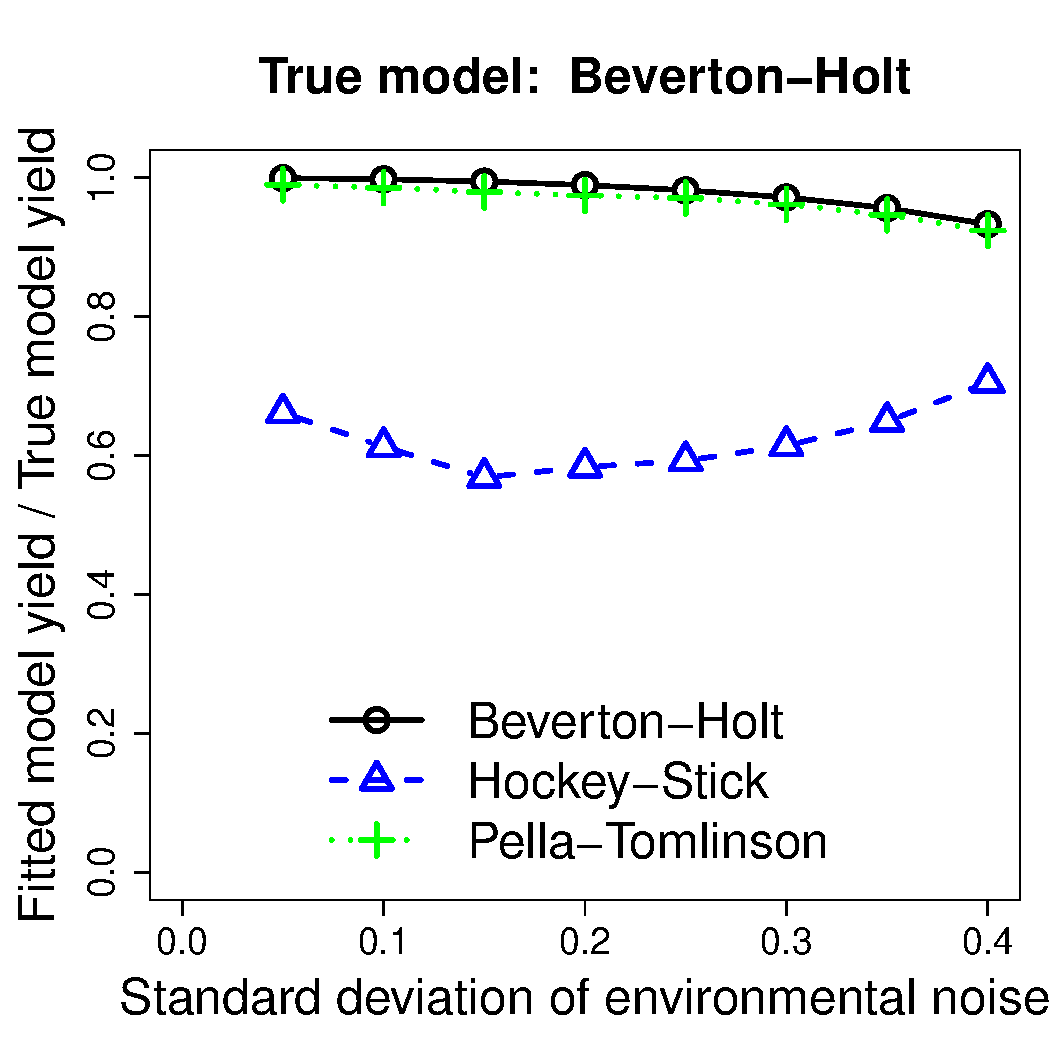
\includegraphics[width=\linewidth,valign=t]{True_1_relativeYield_sim_high_r.pdf}
	\end{subfigure}	
	\begin{subfigure}[t]{0.02\textwidth}
		\textbf{e)}
	\end{subfigure}
	\begin{subfigure}[t]{0.3\textwidth}
		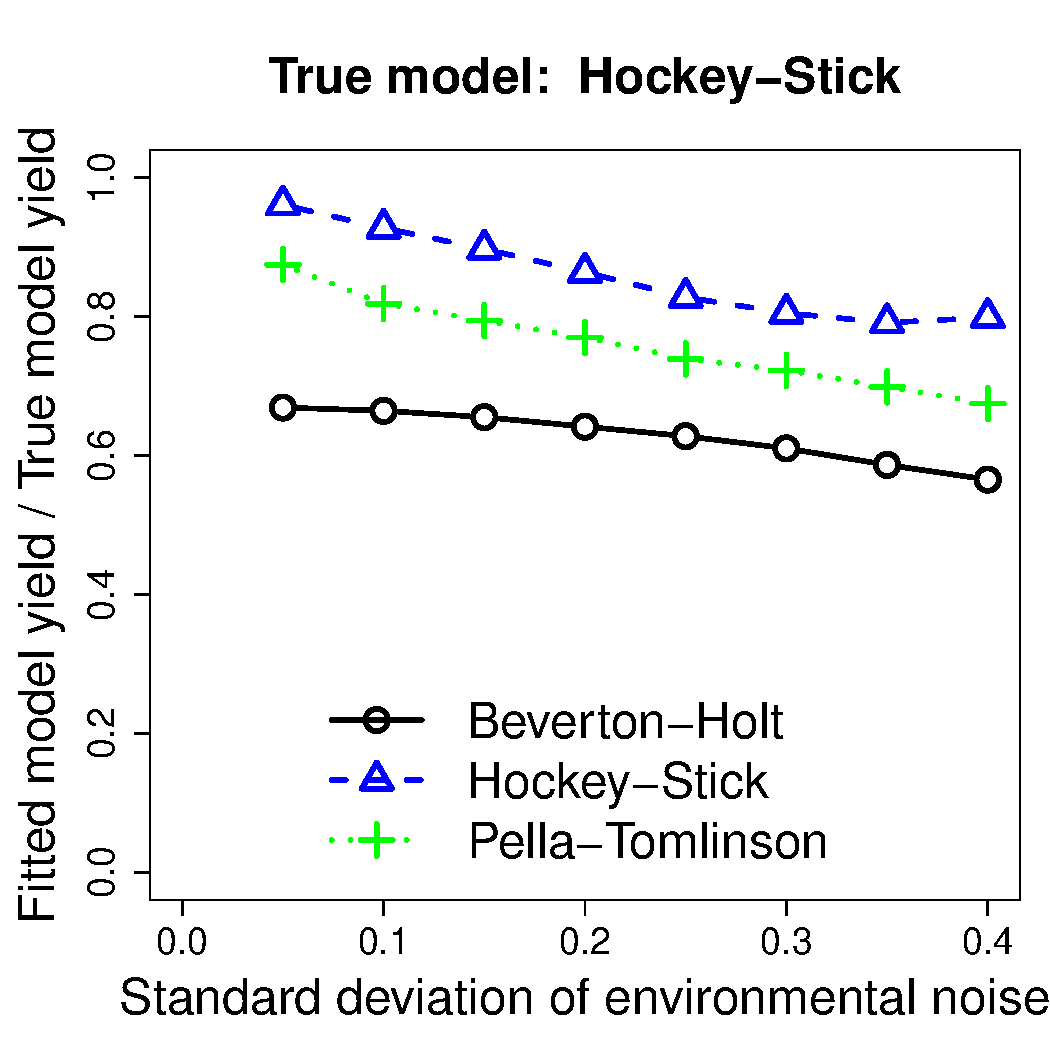
\includegraphics[width=\linewidth,valign=t]{True_2_relativeYield_sim_high_r.pdf}
	\end{subfigure}	
	\begin{subfigure}[t]{0.02\textwidth}
		\textbf{f)}
	\end{subfigure}
	\begin{subfigure}[t]{0.3\textwidth}
		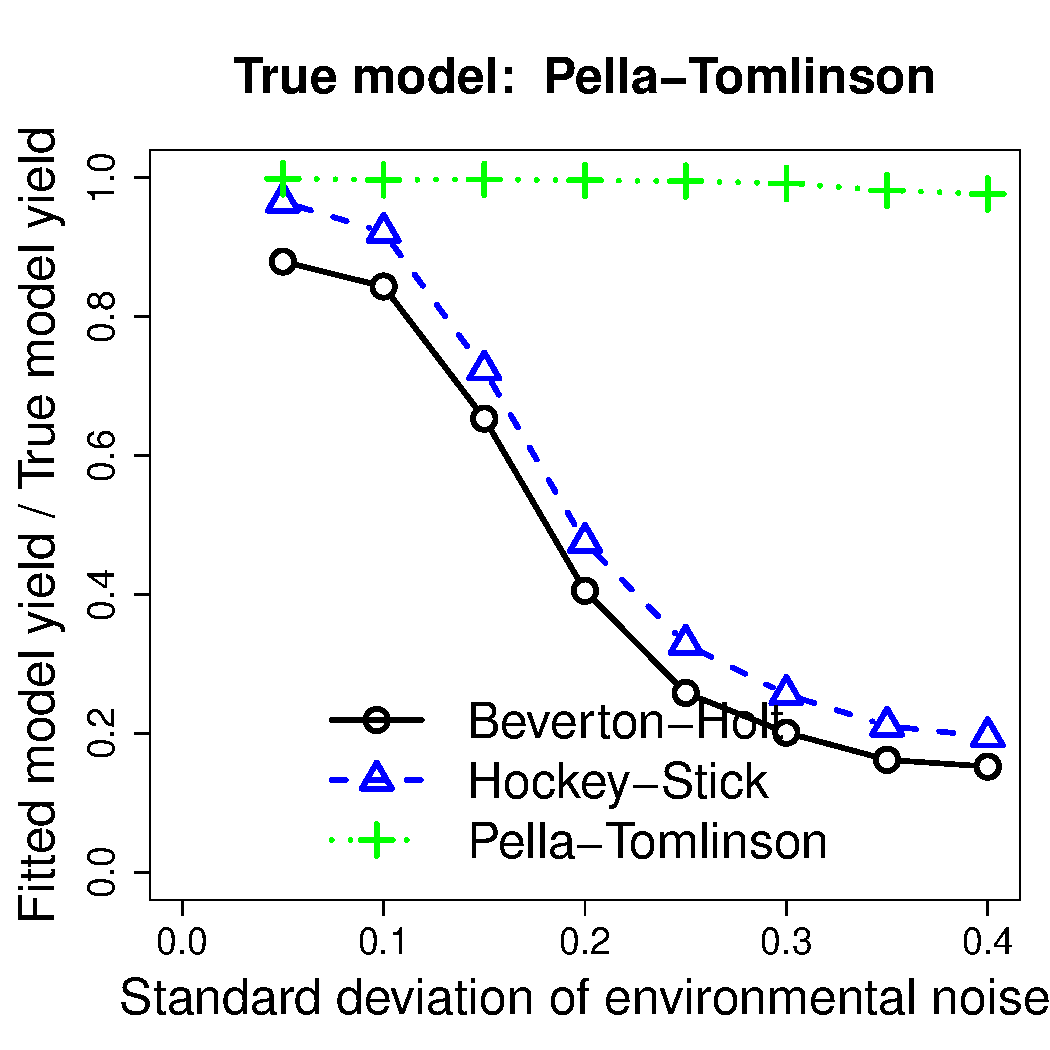
\includegraphics[width=\linewidth,valign=t]{True_3_relativeYield_sim_high_r.pdf}
	\end{subfigure}
	\caption{\textbf{Model Performance under alternative scenarios}. The curves are the means over $1,000$ simulations of harvest yield achieved using the optimal escapement rule produced by a fitted model (circle = Beverton-Holt, triangle = hockey-stick, cross = Pella-Tomlinson) divided by the corresponding yield achieved using the true optimal escapement rule with parameters known, for different values of the standard deviation of the environmental noise. In (row a-c) $r=0.15$, (row d-f) $r=1$. Each column is a different true model. In all plots, $k=100$, and for the Pella Tomlinson model $\phi = 1$.}\label{fig:ModelPerfVSig}
\end{figure}


\section*{References}\label{references}
\bibliography{NearKEscapement}

\addcontentsline{toc}{section}{References}

\hypertarget{refs}{}

\end{document}


